\section{\texorpdfstring{ALU, registr, paměť}{ALU, registr, pamet}}

% =====================================================================================================================
	\begin{frame}
    \frametitle{Aritmeticko-logická jednotka (ALU)}
		\small
		
		\begin{itemize}
			\item Je základní součástí procesoru:
			\begin{itemize}
				\item provádí matematické operace (sčítání, odčítání, násobení, ...),
				\item logické operace (AND, OR, NOT, ...),
				\item bitové posuny a rotace,
				\item pracuje s daty v \textbf{registrech} (STM8 - \textbf{akumulátor}).
			\end{itemize}
				
			\vspace{3mm}
			\item Konkrétní typ operace je určen \textbf{řadičem instrukcí}.
			\item Operandy jsou do registrů načítány po sběrnici z paměti a výsledek operací je ukáldán do určeného registru (STM8 - \textbf{akumulátor}).
			\item Stav výsledku je signalizován příznakovými bity:
			
			\begin{itemize}
				\item \textbf{C} ... přenos,
				\item \textbf{Z} ... nulový výsledek,
				\item \textbf{N} ... záporný výsledek atd.
			\end{itemize}
		\end{itemize}
		
	\end{frame}
	
% =====================================================================================================================
	\begin{frame}
    \frametitle{ALU - příklad}
		\small
		\begin{center}
			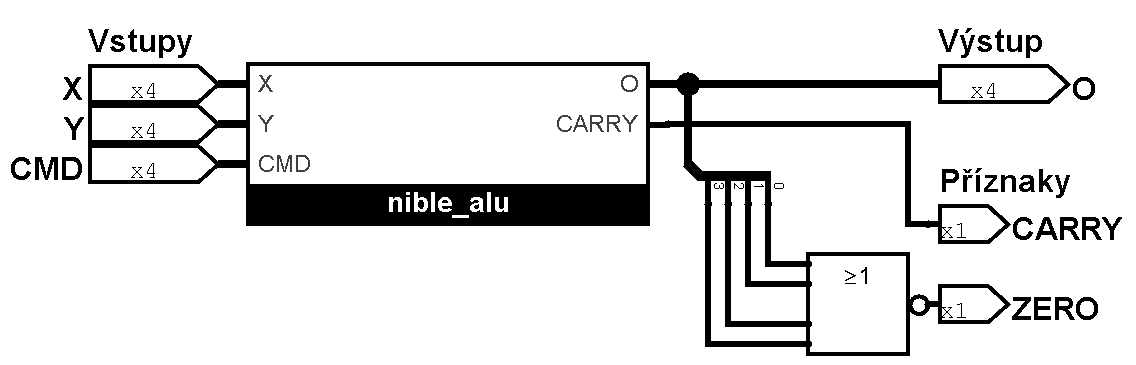
\includegraphics[width=0.70\textwidth]{fig/alu.png}
		\end{center}
		
		\begin{minipage}[t][\textheight][t]{0.48\textwidth}
		
		\textbf{Proměnné:}
		
		\begin{itemize}
			\item \textbf{X,Y} ... operandy,
			\item \textbf{CMD} ... volba operace,
			\item \textbf{O} ... výstup,
			\item \textbf{C, Z} ... příznakové bity.
		\end{itemize}
	
		Logické operace doplňuje možnost negace operandů pomocí bitů 0 a 1 v \textbf{CMD}. 
			
		\end{minipage}
		\begin{minipage}[t][\textheight][t]{0.48\textwidth}
		\vspace{1mm}
		\begin{center}
			\begin{tabular}{| c | l|}
				\hline
				\textbf{CMD} & \textbf{Výstup} \\
				\hline
				$0000$ & $X$ \\
				$0001$ & $\bar{X}$ \\
				$0100$ & $X$ or $Y$ \\
				$1000$ & $X$ and $Y$ \\
				$1100$ & $X + Y$ \\
				$1110$ & $X - Y$ \\
				\hline
			\end{tabular}
		\end{center}
		
		\end{minipage}
		
	\end{frame}
	
% =====================================================================================================================
	\begin{frame}
    \frametitle{ALU - příklad, vnitřní uskupení}
		\small
		\begin{center}
			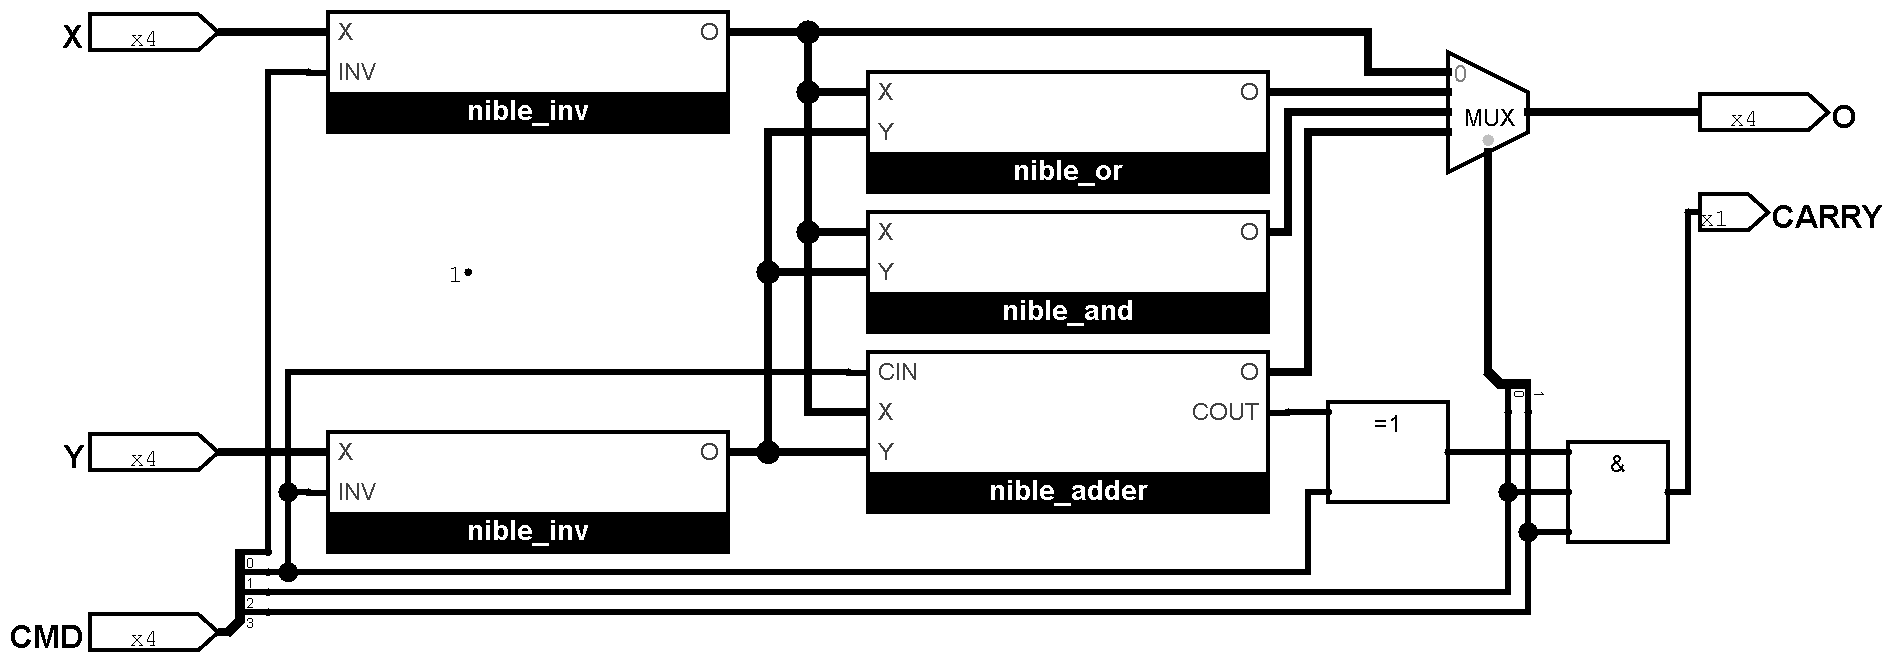
\includegraphics[width=\textwidth]{fig/alu_inside.png}
		\end{center}
		
		\begin{itemize}
			\item Čistě kombinační logika,
			\item \textbf{AND} a \textbf{OR} provádějí operaci mezi příslušnými bity, tj. $X0$ s $Y0$, $X1$ s $Y1$, $X2$ s $Y2$ atd.
		\end{itemize}
	\end{frame}
	
% =====================================================================================================================
	\begin{frame}
    \frametitle{ALU - Počátek vzhledu instrukce}
		
		Návrh Instrukce ve strojovém kódu = binární zápis
		
		\begin{center}
			\begin{tabular}{| c | c | c |}
				\hline
				\textbf{CMD} & \textbf{1. OPERAND} & \textcolor{red}{\textbf{2. OPERAND}}\\
				\hline
			\end{tabular}
		\end{center}
		
		
		\begin{itemize}
			\item Zápis obou operandů v instrukci prodlužuje její délku,
			\item výhodnější je zapsat nejdříve první operand do paměti ALU a pak následně provést požadovanou operaci s přenesením druhého operandu.
		\end{itemize}
		
		\vspace{1mm}
		\textcolor{blue}{\textbf{Registr:}}
		
		\begin{itemize}
			\item Velmi rychlá malá paměť (8, 16, 32 bitů), která je přímo součástí procesoru,
			\item není trvalou paměť, po ztrátě napájení dojde k jejímu vymazání,
			\item často plní specializovaný účel u konkrétní periferie, jako například vstup i výstup aritmetické jednotky.
		\end{itemize}
	\end{frame}

% =====================================================================================================================
	\begin{frame}
    \frametitle{Registr - příklad}
		
		\begin{minipage}[t][\textheight][t]{0.48\textwidth}
		
		\textbf{Ukázka:}
		\begin{center}
			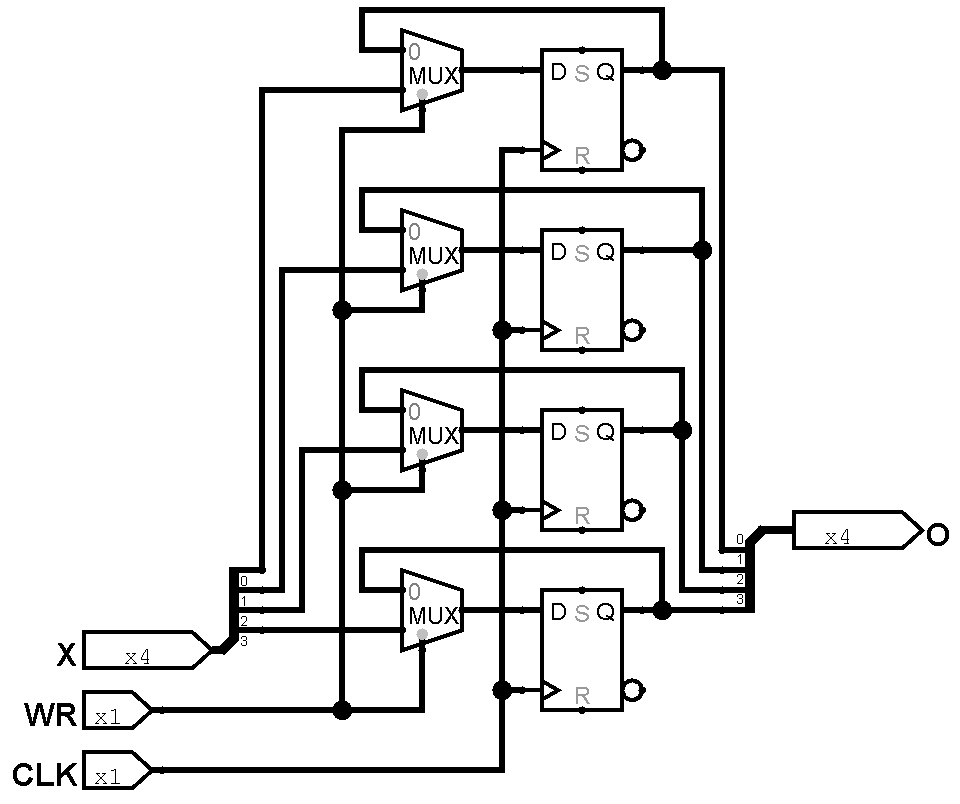
\includegraphics[width=\textwidth]{fig/register.png}
		\end{center}
			
		\end{minipage}
		\begin{minipage}[t][\textheight][t]{0.48\textwidth}
		\small
		\vspace{1mm}
		\begin{itemize}
			\item 4 bit registr,
			\item synchronní zápis na hranu hodin,
			\item zápis se povoluje $WR = 1$,
			\item toto je logická reprezentace, nejedná se o skutečné provedení uvnitř CPU.
		\end{itemize}
		\vspace{2mm}
		\begin{center}
			\begin{tabular}{c c | c}
				\hline
				$CLK$ & $WR$ & $OUT$ \\
				\hline
				$\uparrow$ & $0$ & $OUT$ \\
				$\uparrow$ & $1$ & $X$ \\
			\end{tabular}
		\end{center}
		
		\end{minipage}
	\end{frame}
	
% =====================================================================================================================
	\begin{frame}
    \frametitle{Registr - akumulátor příklad}
		
		\begin{minipage}[t][\textheight][t]{0.55\textwidth}
		
		\textbf{Ukázka:}
		\begin{center}
			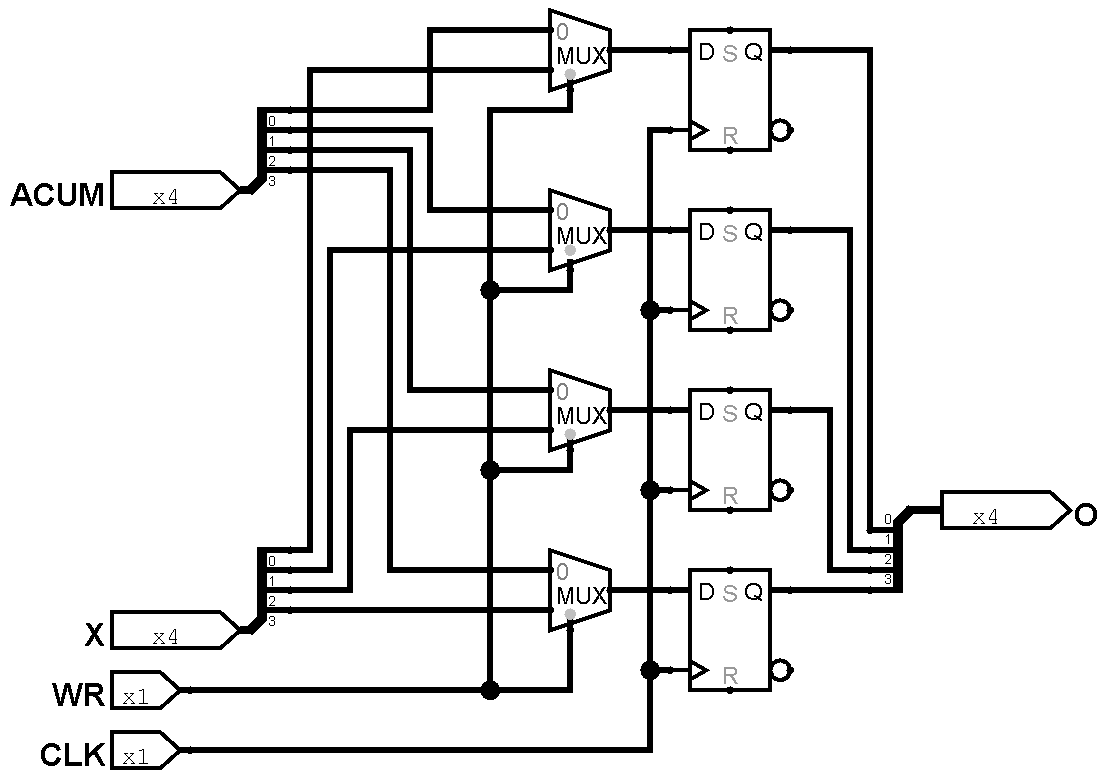
\includegraphics[width=\textwidth]{fig/acumulator.png}
		\end{center}
			
		\end{minipage}
		\begin{minipage}[t][\textheight][t]{0.4\textwidth}
		\small
		\vspace{1mm}
		\begin{itemize}
			\item Zpětná vazba pro uchování hodnoty je jako vstup,
			\item jinak je zapojení stejné jako předchozí.
		\end{itemize}
		
	  \vspace{3mm}
		Vstup \textbf{ACUM} použijeme pro zápis výsledku z \textbf{ALU}.
		
		\end{minipage}
	\end{frame}
	
% =====================================================================================================================
	\begin{frame}
    \frametitle{ALU s akumulátorem}
		
		\begin{center}
			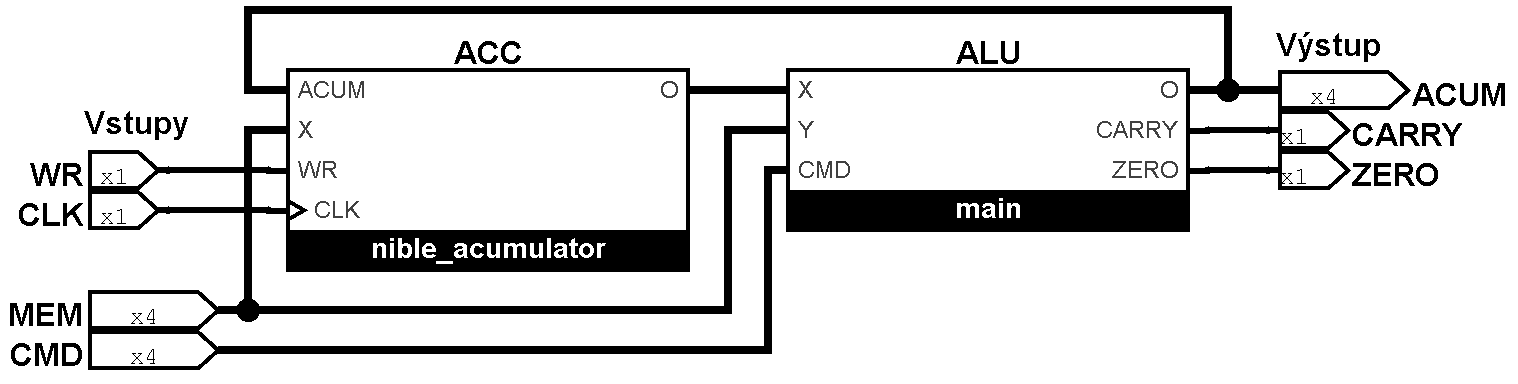
\includegraphics[width=0.9\textwidth]{fig/alu_acum.png}
		\end{center}
		
		
		\begin{itemize}
			\item Registr \textbf{ACC} tvoří jak jeden z operandů, tak cílovou paměť pro uložení výsledku.
			\item Druhý operand se načítá ze sběrnice (\textbf{MEM}), kde je buď obsah paměti nebo jiného registru.
			\item Každá \textbf{ALU} má registr s podobnou funkcí. Nicméně, název registru akumulátor (nebo střadač) je specifický pro procesory STM8.
		\end{itemize}
		
	\end{frame}
	
% =====================================================================================================================
	\begin{frame}
    \frametitle{Ukázka aritmetických a logických instrukcní STM8}
		\small
		\begin{center}
			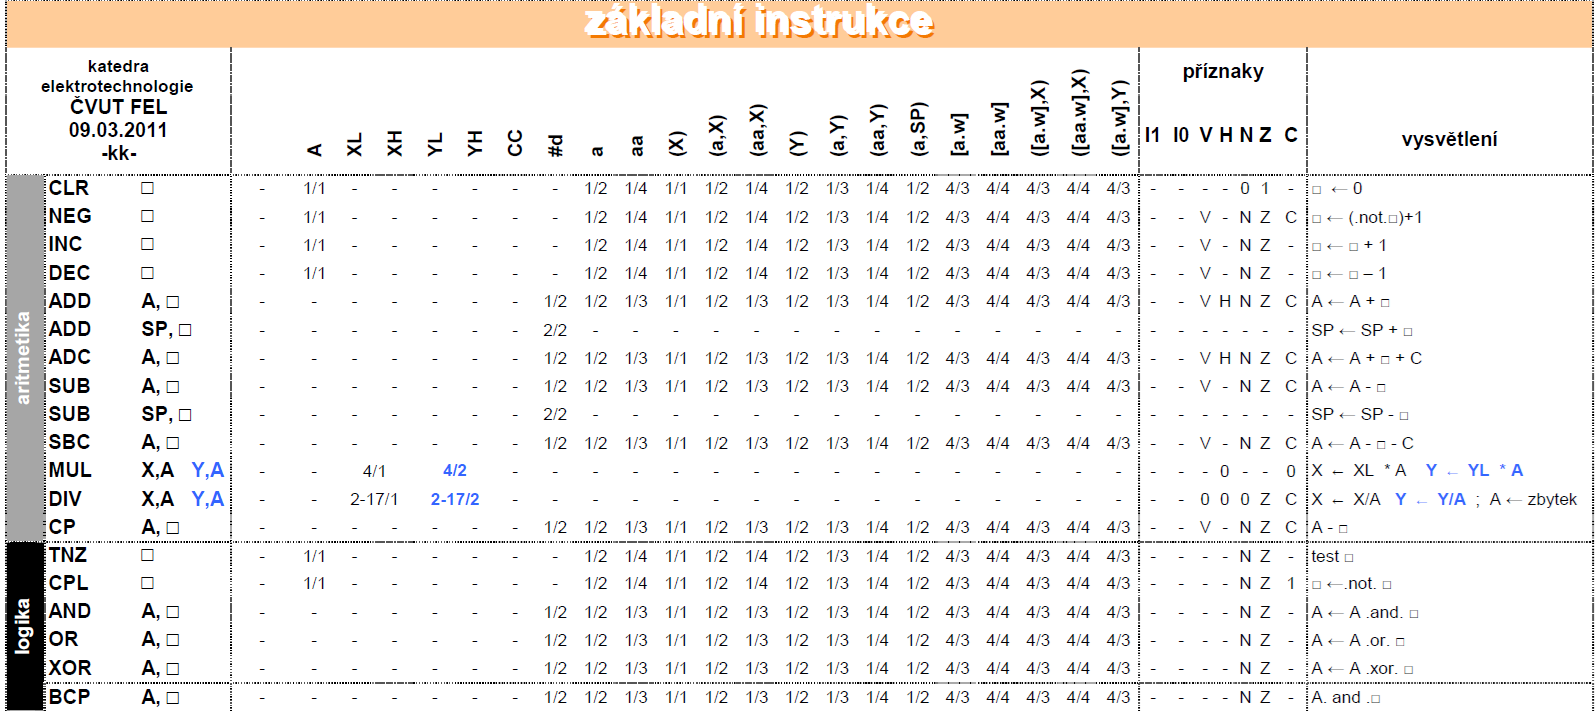
\includegraphics[width=\textwidth]{fig/instr_example.png}
		\end{center}
		
		
		\begin{itemize}
			\item Akumulátor je součástí všech aritmetických i logických instrukcí assembleru STM8.
		\end{itemize}
		
	\end{frame}
	
% =====================================================================================================================
	\begin{frame}
    \frametitle{Paměť}
		\small
		
		\begin{center}
			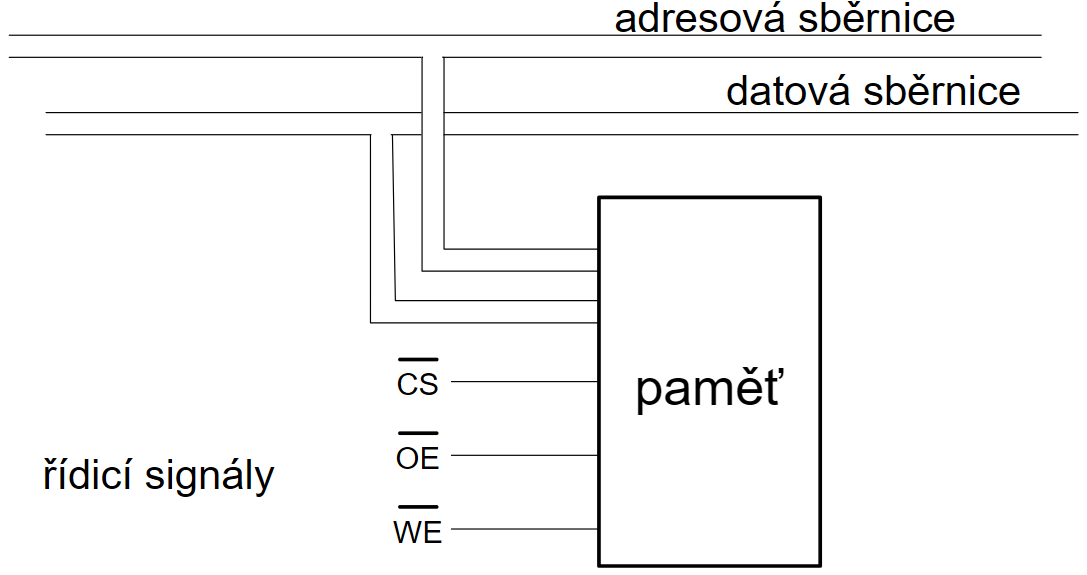
\includegraphics[width=0.55\textwidth]{fig/memory.png}
		\end{center}
		
		\begin{itemize}
			\item Registry jsou nevhodné pro záznam většího množství dat, kvůli relativní složitosti paměťové jednotky (velikost, integrace),
			
			\item paměťová buňka je výrazně jednodušší,
			\item pro její obsluhu využíváme:
			
			\begin{itemize}
				\item adresovou sběrnici pro nastavení buňky s daty,
				\item datovou sběrnici pro zápis a čtení obsahu buňky a
				\item řídící signály pro kontrolu zápisu, přístupu na sběrnici apod.
			\end{itemize}
		\end{itemize}
		
	\end{frame}
	
% =====================================================================================================================
	\begin{frame}
    \frametitle{Paměť - STM8}
		\small
		\begin{minipage}[t][\textheight][t]{0.8\textwidth}
		
		\begin{itemize}
			\item Paměť dělíme na:
			
			\begin{itemize}
				\item trvalou (nevolatilní), která uchovává data i po ztrátě napájení a
				\item dočasnou (volatilní), která data ztratí se ztrátou napájení.
			\end{itemize}
		\end{itemize}
		
		\vspace{2mm}
		V případě procesorů řady STM8 je k dispozici paměť:
		
		\begin{itemize}
			\item \textbf{ROM, FLASH} - trvalá paměť určená pro zápis programu, přepisuje se po blocích.
			\item \textbf{EEPROM} - trvalá paměť určená pro zálohování dat programu, přepisuje se po jednotkách.
			\item \textbf{RWM = RAM} - volatilní paměť určená pro práci s daty, velmi rychlá.
		\end{itemize}
			
		\end{minipage}
		\begin{minipage}[t][\textheight][t]{0.12\textwidth}
		\tiny
		\begin{center}
		\textbf{STM8}
			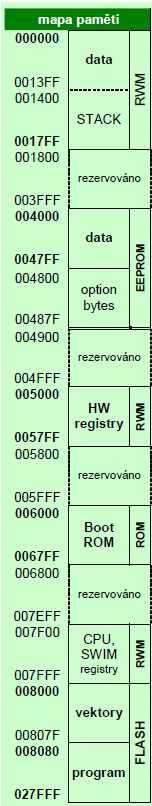
\includegraphics[width=0.9\textwidth]{fig/memory_STM8.png}
		\end{center}
		
		\end{minipage}
		
	\end{frame}